\chapter{Билет №7}

\section*{Классификация типов ввода-вывода с точки зрения программиста: диаграммы последовательности действий для каждого типа ввода-вывода и описание. Классификация моделей ввода-вывода. Особенности и назначение асинхронного ввода-вывода. Мультиплексирование. Пример мультиплексирования для сокетов \\AF\_INET, SOCK\_STREAM. Сетевой стек. Пример (лаб. раб.)}

\section{Классификация типов ввода-вывода с точки зрения программиста}
\begin{quote}
\textbf{Идея распараллеливания функций}

С оперативной памятью мы работаем при помощи команды mov, а с внешними устройствами - через порты ввода вывода командами in и out. (memory mapping, io mapping)

60-е - начало 70-х - появление интегральных микросхем, позволивших значительно увеличить мощности вычислительной системы, уменьшить её габариты.

В машинах ibm360,370 была реализована идея распараллеливания функицй.

Так как процессор всегда был самым быстродействующим устройством системы и это стало их отличительной чертой. Внешние устройства - механика, медленные устройства.

Чтобы более эффективно использовать процессорное время, была реализована архитектура с распараллеливанием функций: в состав ibm360 были включены специальные процессоры-каналы, которые взяли на себя функцию усправления внешними устройствами.

Таким образом, процессор был освобождён от усправления внешними устройствами, но это требовало реализации в системе полноценной системы прерываний: процессор инициализирует ввода-выывода, а управляет ей канал. По завершении операции ввода-вывода прерывание информирует провессор о завершении данной операции - это основа функционирования любой системы.

В ПК на базе intel - шинная архитектура.

Архитектура мейнфреймов ibm называется канальной.

В шинной архитектуре внешними устройствами управляют специальные устройства - контроллеры.

Основное отличие асинхронного ввода-вывода от ввода-вывода, управляемого сигналом: при вводе-выводе, управляемым сигналом, сигнал информирует процесс и готовности данных, а при асинхронном вводе-выводе процесс вообще не блокируется и информируется о полном завершении операции ввода-вывода.
\end{quote}
\subsection{Блокирующий синхронный ввод-вывод}
Блокирующий ввод-вывод (запрос на получение данных read). Используется ключевое слово receive from – общее средство передачи данных в системе.
Передача данных с помощью сообщений – самый общий способ, который может рассматриваться как на отдельно стоящей машине, так и в распределенной системе. 

receive from = запрос на получение данных = read. Все сводится к системным вызовам read/write.

send to/receive from, как и read/write, переводят систему в режим ядра, так как это системные вызовы.

Процесс, выполнивший системный вызов ввода-вывода (не важно, read или write), будет ожидать ошибки, либо значение, соответствующее успешному выполнению системного вызова.

То есть процесс в любом случае получит данные (в случае read/receive from это особенно явно).
\subsection{Блокирующий ввод-вывод (blocking)}
\begin{table}[H]
  \centering
  \begin{tabular}{p{1\linewidth}}
    \centering
    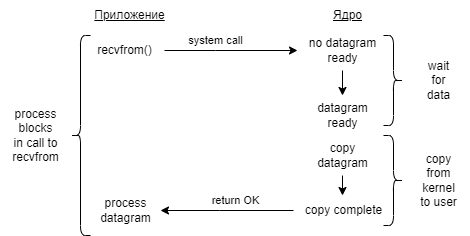
\includegraphics[width=0.8\linewidth]{./images/1-1.png}
  \end{tabular}
\end{table}
Когда приложение выполняет запрос ввода-вывода (в примере ввод – receive from), процесс блокируется до тех пор, пока не получит данные.

Что значит datagram ready (данные готовы)? Если мы вводим символ с клавиатуры, то он готов тогда, когда он введен в буфер клавиатуры.

Далее он копируется в буфер ядра, и уже оттуда в буфер приложения, после чего оно сможет продолжить свое выполнение.

\begin{quote}
Системы реального времени работают в готовыми данными (с датчиков из измерительных приборов, считавших показания). Данные готовы, их нужно только получить. Если данные не готовы, будет возвращена ошибка, то есть мы не можем обработать соответствющие данные, и надо выполнить доп. действия. Надо понимать, когда это возможно, а когда нет.
\end{quote}

\begin{quote}
Диаграмма из 1 вопроса на запрос ввода вывода + пояснения
\end{quote}

Таким образом, весь ввод – вывод который мы реализовывали в своих программах, является блокирующим (пока процесс не получит данные, он будет заблокирован). 

Такой ввод-вывод возможен, только если в системе реализованы аппаратные прерывания, то есть прерывания от внешних устройств. 

В современных системах для отдельно стоящей машины блокирующий ввод-вывод – основная модель ввода-вывода (запросив ввод-вывод, приложение блокируется, система переходит в режим ядра и запрос обслуживается).

При этом в блокирующем вводе-выводе в полной мере реализована идея распараллеливания функций (3-е поколение ЭВМ), которая базируется на стремлении освободить процессор от непроизводительных действий (управляется медленными внешними устройствами).

Пока медленное внешнее устройство выполняет задачу ввода данных, процессор может перейти на выполнение другой работы.

\subsection{Неблокирующий ввод-вывод}

Исторически был реализован раньше блокирующего. Управление операцией ввода-вывода осуществляет процессор: он опрашивал флаг устройства, который информировал процессор о готовности данных.
\begin{table}[H]
  \centering
  \begin{tabular}{p{1\linewidth}}
    \centering
    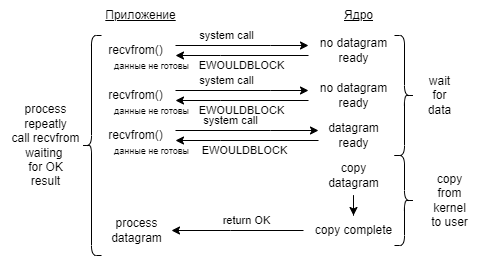
\includegraphics[width=0.8\linewidth]{./images/1-2.png}
  \end{tabular}
\end{table}

Опрос (polling) – периодическое действие: опрос выполняется до тех пор, пока данные не будут готовы, то есть пока они не поступили в буфер ядра и из него уже в буфер приложения.

При этом процесс не блокируется, но процессорное время тратиться на опрос. 

E-Error: ошибка обращения, данные не готовы.

Для этого определяется специальные возвращаемые значения для каждой конкретной модели ввода-вывода. Это учитывается разработчиками системы.

Здесь нет аналогии с активным ожиданием на процессоре: это концептуально разные вещи. В данном случае идет опрос флага о готовности контроллера прерывания, то есть это обращение к внешнему устройству.

В система должны быть специальные команды для работы в режиме polling, однако это устаревший способ взаимодействовать с внешними устройствами. Он затраный, но исключить опрос для любой системы мы не можем, В каких-то системах допускается возможность реализации такого опроса, а в наших – нет, так как у нас есть прерывания от внешних устройств (блокрующий ввод-вывод).

\subsection{Мультиплексирование ввода-вывода}

Мультиплексирование всегда рассматривается для модели «клиент-сервер» на соекетах. Этот способ выделяется как самостоятельная модель ввода-вывода без привязки к сокетам.                                                  

Мультиплексирование – очень хорошая альтернатива многопоточности. Многопоточность очень затратная, особенно на UNIX/Linux (а Windows заточен на потоки, а не на процессы).

Для реализации мультиплексирования система предоставляет специальные системные вызовы (мультиплексеры) select и poll.

select() == pselect()

poll() == epoll() в современных системах.

Сокеты – тоже альтернатива многопоточности.

\begin{table}[H]
  \centering
  \begin{tabular}{p{1\linewidth}}
    \centering
    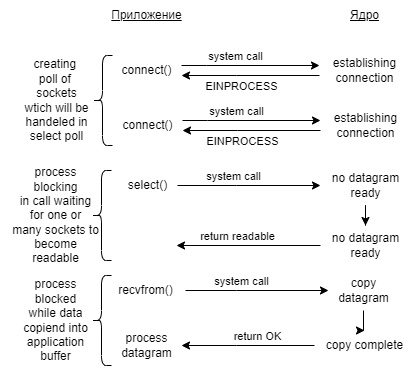
\includegraphics[width=0.8\linewidth]{./images/1-3.png}
  \end{tabular}
\end{table}
Формируется пул сокетов, которые будут обрабатываться в петле select.

На select сервер будет длокирован, но время блокировки будет меньше, так как опрашивается сразу пул сокетов. Вероятность готовности какого-то либо сокета из множества выше вероятности готовности конкретного сокета.

Взаимодействие так же выполняется путем передачи сообщений, но receive from выкинули, иначе диаграмма была бы слишком большой. Поэтому указывается только select.

Мультиплексирование используется только для сетей (распределенных систем).

Мультиплексирование позволяет сократить время блокировки (блокировки – зло, но зло неизбежное) за счет того, что мультиплексор фактически опрашивает готовность точек соединения (на своей стороне, так как клиенты устанавливают соединение с сервером).

Время ожидания готовности одной точки соединения из пула точек соединения будет меньше времени ожидания соединения в определенном порядке.

Взаимодействие на сокетах осуществляется по модели клиент-сервер: сервер предоставляет ресурсы и службы одному или нескольким клиентам, которые обращаются к серверу за обслуживанием. 

В момент, когда клиент запрашивает соединение с сервером, сервер может либо принять, либо отклонить запрос на соединение. Если соединение устанавливается, то оно поддерживается по определённому протоколу.

После того, как select определил, что соединение установлено, вызывается receive from.

Когда данные готовы, возвращается readable (данные доступны), вызывается receive from и производится копирование из буфера ядра в буфер приложения.

process datagram – обработка данных.

select вызывается на стороне сервера, сервер однопоточный, так как мультиплексирование – альтернатива многопоточности.

Пример мультиплексора – переключатель режимов работы стиральной машины.

\subsection{Ввод-вывод, управляемый сигналом}

\begin{table}[H]
  \centering
  \begin{tabular}{p{1\linewidth}}
    \centering
    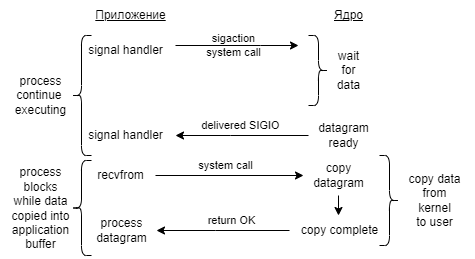
\includegraphics[width=0.8\linewidth]{./images/1-4.png}
  \end{tabular}
\end{table}

Устанавливается обработчик специального сигнала SIGIO, задача которого – проинформировать процесс о том, что данные готовы (delivered SIGIO – доставка сигнала процессу).

Процесс вызывает receive from, чтобы получить данные.

Буфер устройства → Буфер ядра → Буфер приложения.

Процесс продолжает выполняться и блокируется только на время копирования данных, то есть время блокировки уменьшилось.

Всю работу в данном способе ввода-вывода берет на себя ядро: оно отслеживает готовность данных и после этого посылает сигнал SIGIO. В результате будет вызван обработчик этого сигнала.

Это (обработчик) называется callback-функцией (функцией обратного вызова).

При этом receive from можно выполнить либо в обработчике сигнала, либо в главном потоке программы.

Сигнал типа SIGIO для каждого процесса может быть только один.

В результате в каждый момент времени можно работать только с одним файловым дескриптором.

На время выполнения обработчика сигнала данный сигнал блокируется.

Если в период блокировки доставляются несколько сигналов, то они теряются.

Если маска сигнала (sa\_mask) установлена в NULL, то на время выполнения обработчика сигнала другие сигналы не блокируются.

\subsection{Асинхронный ввод-вывод}

Блокировки увеличивают время выполнения приложения, время блокировки – случайная величина. Разработчики стремятся избежать блокировок и системы предоставляют соответствующие системные вызовы, обеспечивающие асинхронный ввод-вывод. 

Для его реализации система предоставляет пользователю специальные системные вызовы. Как правило, они начинаются с a – asynchronous.

\begin{table}[H]
  \centering
  \begin{tabular}{p{1\linewidth}}
    \centering
    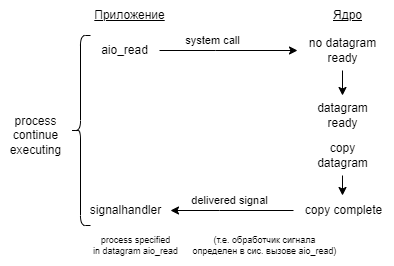
\includegraphics[width=0.8\linewidth]{./images/1-5.png}
  \end{tabular}
\end{table}

Процесс не блокируется и продолжает выполняться. В отличие от предыдущей модели, сигнал информирует процесс о полном завершении операции ввода-вывода, включая копирование данных. 

Здесь вместо receive from используется read/write, так как здесь нет передачи сообщений, это в чистом виде ввод-вывод на отдельно стоящей машине. 

receive from/send to – системные вызовы, связанные с приемом/посылкой сообщений.
read/write – системные вызовы, связанные с получением данных от внешних устройств (по факту из файла, так как в UNIX все файл).

Асинхронный ввод-вывод определен в POSIX (спецификация POSIX, согласовавшая все различия в функциях осинхронного ввода-вывода, возникших в разных системах, объединив их достоинства.

Все функции асинхронного ввода/вывода работают таким образом, что они сообщают ядру о начале операции ввода-вывода, а процесс они уведомляют о завершении операции ввода-вывода, включая копирование данных.

Основное отличие асинхронного ввода-вывода от ввода-вывода, управляемого сигналом: при вводе-выводе, управляемым сигналом, сигнал информирует процесс и готовности данных, а при асинхронном вводе-выводе процесс вообще не блокируется и информируется о полном завершении операции ввода-вывода.

Проблема асинхронного ввода-вывода: необходимо получать асинхронные события синхронно, так как данные нужны приложению для выполнения дальнейших действий.

В асинхронном вводе-выводе внимание сосредотачивается на 2 моментах:
\begin{enumerate}
\item На возможности определить, что ввод-вывод можно выполнить быстро (в технике нет быстро/медленно);
\item На завершении операции ввода-вывода в случае невозможности немедленного выполнения ввода-вывода, то есть возвращения ошибки.
\end{enumerate}

\subsection{Классификация моделей ввода-вывода}

\begin{table}[]
\begin{tabular}{|l|l|l|}
\hline
            & Blocking                                                                                                        & Non-blocking                                                  \\ \hline
Synchronous & \begin{tabular}[c]{@{}l@{}}1) recv from / send to /read /write\\  - в разных источниках по-разному\end{tabular} & \begin{tabular}[c]{@{}l@{}}2) polling\\  (опрос)\end{tabular} \\ \hline
Asynchonous & \begin{tabular}[c]{@{}l@{}}3) IO multiplexing \\ 4) SIGIO\end{tabular}                                          & 5) AIO                                                        \\ \hline
\end{tabular}
\end{table}

\section{Сетевой стек}

Сети ~ распределенные системы, т.е. у каждого хоста своя память

В сетях - только передача сообщений, которые должны сопровождаться адресом

Пакет - сообщение с адресом + служебная информация 

В Linux определен интерфейс между пользовательскими процессами и стеком сетевых протоколов в ядре.

\begin{quote}
Это не по семинару*

Модули протоколов группируются по семействам протоколов, такими, как AF\_INET, AF\_IPX и AF\_PACKET, и типам сокетов, такими, как SOCK\_STREAM или SOCK\_DGRAM. Сетевой стек ядра Linux имеет две структуры:

struct socket — интерфейс высокого уровня, который используется для системных вызовов (именно поэтому он также имеет указатель struct file, который представляет файловый дескриптор)

struct sock — реализация в ядре для AF\_INET сокетов (есть также struct unix\_sock для AF\_UNIX сокетов, которые являются производными от данного), которые могут использоваться как в ядре, так и в режиме пользователя.
\end{quote}

\begin{table}[H]
  \centering
  \begin{tabular}{p{1\linewidth}}
    \centering
    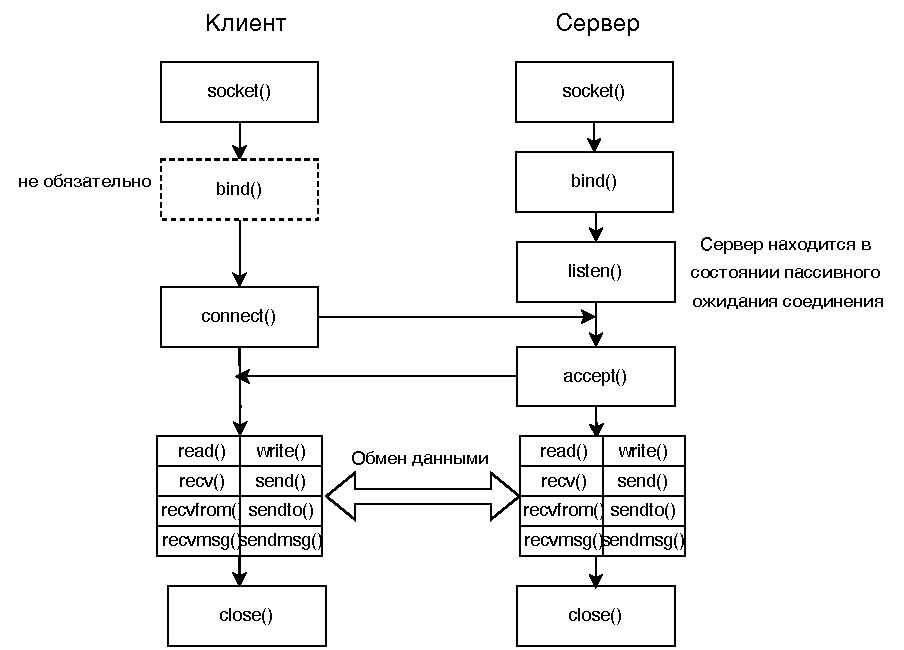
\includegraphics[width=0.8\linewidth]{./images/4.pdf}
  \end{tabular}
\end{table}

socket() - создание точки соединения. Возвращает файловый дескриптор. Сокет - специальный файл (у него есть inode), назначение которого - обеспечивать соединения;

AF\_INET, SOCK\_STREAM - сетевое взаимодействие по протоколу TCP

bind() связывает сокет с адресом (сетевым (порт + API-адрес) в случае сокетов AF\_INET)

\begin{lstlisting}
int bind(int sockfd, struct sockaddr *addr, int addrlen);
\end{lstlisting}

struct sockaddr\_in - есть поле “порт” и “сетевой адрес” (у них должен быть сетевой порядок (применяем функцию htons())

На сервере вызов bind() обязателен, на клиенте нет, т.к. его точный адрес часто не играет никакой роли (если bind() не вызывается, адрес назначается клиентам автоматически)

listen() информаирует ОС о том, что он готов принимать соединения (имеет смысл только для протоколов, ориентированных на соединение (например, TCP)

\begin{lstlisting}
int listen(int sockfd, int baclog);
\end{lstlisting}
connect() - клиент устаналивает активное соединение с сокетом (с сервером)
\begin{lstlisting}
int connect(int sockfd, struct sockaddr *addr, int addrlen)
\end{lstlisting}

Для протокола без соединения (например, UDP) connect может использоваться для указания адреса назначения всех передаваемых пакетов

accept() - вызывается на стороне сервера, если соединение установлено. Сервер принимает соединение, *только если* он получил запрос на соединение.

\begin{lstlisting}
int accept(int sockfd, void* addr, int *addrlen)
\end{lstlisting}

Когда соединение принимается, accept()  создает копию исходого сокета, чтобы сервер мог принимать другие соединения. Исходный сокет остается в состоянии listen, а копия будет находиться в состоянии connected. accept() возвращает файловый дескриптор копии исходного сокета.

\begin{quote}
про уровни сетевых протоколов

Протоколы различаются по уровням. Нижний уровень - непосредсвенное взаимодействие с аппаратной частью (самое важное)
\end{quote}

\section{Пример мультиплексирования для сокетов  AF\_INET, SOCK\_STREAM (лаб. раб.)}

Сетевые сокеты с мультиплексированием:

Мультиплексирование - альтерната многопоточности (созданию дочернего процесса/потока для обработки каждого соедниния)

\begin{table}[H]
  \centering
  \begin{tabular}{p{1\linewidth}}
    \centering
    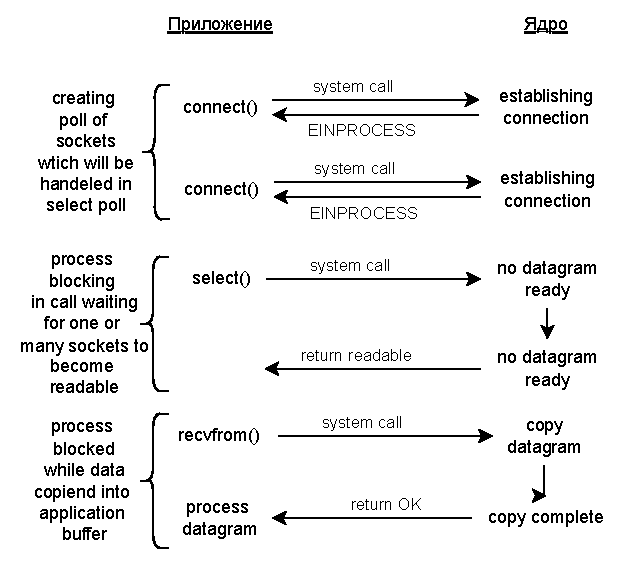
\includegraphics[width=0.8\linewidth]{./images/7-2.pdf}
  \end{tabular}
\end{table}

\begin{quote}
Это детализированная схема: клиенты вызывают connect() и создается пул сокетов.

Для сокращения времени блокировки сервера в ожидании соединения используется select() (пока соединение не возникнет, сервер будет блокирован на accept(), т.е. будет в состоянии пассивного ожидания соединения), т.к. время установления соединения со многими клиентами меньше, чем с каждым конкретным клиентом в определенной последовательности.

В результате select() создает пул соединение. Есть макрос, который “реагирует” на возникновение хотя бы одного соединения. В результате будет вызан accept(), который последовательнос принимает соединения.

Для создания пула соединений можно использовать массив.

Мультиплексор опрашивает соединения. Когда соединение готово, оно фиксируется ядром.

Мультиплексопы: 
select    pool
pselect   epool
\end{quote}

Код клиента
\begin{lstlisting}
#include <stdio.h>
#include <stdlib.h>
#include <sys/types.h>
#include <sys/socket.h>
#include <netinet/in.h>
#include <netdb.h>
#include <string.h>
#include <unistd.h>
#include <fcntl.h>
#include <errno.h>

#define SERVER_PORT 8080
#define MSG_LEN 64

int main(void)
{
  setbuf(stdout, NULL);

  struct sockaddr_in serv_addr =
  {
    .sin_family = AF_INET,
    .sin_addr.s_addr = INADDR_ANY,
    .sin_port = htons(SERVER_PORT)
  };
  socklen_t serv_len;

  char buf[MSG_LEN];

  int sock_fd = socket(AF_INET, SOCK_STREAM, 0);
  if (sock_fd == -1)
    // error handling

  if (connect(sock_fd, (struct sockaddr *)&serv_addr, sizeof(serv_addr)) < 0)
    // error handling

  char input_msg[MSG_LEN], output_msg[MSG_LEN];
  sprintf(output_msg, "%d", getpid());

  if (write(sock_fd, output_msg, strlen(output_msg) + 1) == -1)
    // error handling

  printf("Client send:    %d\n", getpid());

  if (read(sock_fd, input_msg, MSG_LEN) == -1)
    // error handling

  printf("Client receive: %s \n", input_msg);
  close(sock_fd);
  return EXIT_SUCCESS;
}
\end{lstlisting}

Код сервера
\begin{lstlisting}
#include <stdlib.h>
#include <stdio.h>
#include <signal.h>
#include <sys/socket.h>
#include <netinet/in.h>
#include <string.h>
#include <unistd.h>
#include <fcntl.h>
#include <errno.h>
#include <sys/epoll.h>

#define MAX_EVENTS_COUNT 100
#define SERVER_PORT 8080
#define MSG_LEN 64

static int sock_fd_global;

void server_shutdown(int signum)
{
    printf("\nShutdowning server...\n");
    close(sock_fd_global);
    exit(EXIT_SUCCESS);
}

int handle_event(int sock_fd)
{
  struct sockaddr_in client_addr; 
  socklen_t client_len;
  char input_msg[MSG_LEN];
  
  int bytes = read(sock_fd, input_msg, MSG_LEN);

  if (bytes == 0)
    return(EXIT_SUCCESS);

  if (bytes == -1)
  {
    perror("read");
    return EXIT_FAILURE;
  }

  printf("Server receive: %s \n", input_msg);

  char output_msg[MSG_LEN];
  sprintf(output_msg, "%s %d", input_msg, getpid());

  if (write(sock_fd, output_msg, MSG_LEN) == -1)
    // error handling

  printf("Server send:    %s \n", output_msg);

  return EXIT_SUCCESS;
}

int main(void)
{
  setbuf(stdout, NULL);

  struct epoll_event ev, events[MAX_EVENTS_COUNT];
  int listen_sock, nfds, epoll_fd;

  struct sockaddr_in serv_addr =
  {
    .sin_family = AF_INET,
    .sin_addr.s_addr = INADDR_ANY,
    .sin_port = htons(SERVER_PORT)
  };
  
  listen_sock = socket(AF_INET, SOCK_STREAM, 0);
  if (listen_sock == -1)
    // error handling
  sock_fd_global = listen_sock;

  if (bind(listen_sock, (struct sockaddr *)&serv_addr, sizeof(serv_addr)) == -1)
    // error handling

  if (listen(listen_sock, 1) == -1)
    // error handling

  signal(SIGINT, server_shutdown);
  signal(SIGTERM, server_shutdown);
  printf("Server is working.\n(Press Ctrl+C to stop)\n");

  epoll_fd = epoll_create1(0);
  if (epoll_fd == -1)
    // error handling

  ev.events = EPOLLIN;
  ev.data.fd = listen_sock;
  if (epoll_ctl(epoll_fd, EPOLL_CTL_ADD, listen_sock, &ev) == -1)
    // error handling

  for (;;)
  {
    nfds = epoll_wait(epoll_fd, events, MAX_EVENTS_COUNT, -1);
    if (nfds == -1)
      // error handling

    for (int n = 0; n < nfds; ++n)
    {
      if (events[n].data.fd == listen_sock)
      {
        struct sockaddr client_addr; 
        socklen_t client_len;
        
        int conn_sock = accept(listen_sock, (struct sockaddr *)&client_addr, &client_len);
        if (conn_sock == -1)
          // error handling
        
        int status = fcntl(conn_sock, F_SETFL, fcntl(conn_sock, F_GETFL, 0) | O_NONBLOCK);
        if (status == -1)
          // error handling

        ev.events = EPOLLIN | EPOLLET;
        ev.data.fd = conn_sock;
        if (epoll_ctl(epoll_fd, EPOLL_CTL_ADD, conn_sock, &ev) == -1)
          // error handling
      }
      else if (handle_event(events[n].data.fd) != EXIT_SUCCESS)
      {
        close(listen_sock);
        exit(EXIT_FAILURE);
      }
    }
  }

  close(listen_sock);
  return EXIT_SUCCESS;
}
\end{lstlisting}